% ============================================ %

\documentclass[14pt,a4paper]{extarticle}
%\documentclass[12pt,a4paper]{article}

\usepackage[utf8]{inputenc}
\usepackage[ukrainian]{babel}
\usepackage[active]{srcltx}
\usepackage[final]{pdfpages}
\usepackage[hidelinks]{hyperref}

\usepackage{verbatim}
\usepackage{amssymb}
\usepackage{physics}
\usepackage{amsmath}
\usepackage{algpseudocode}
\usepackage{algorithm}
\floatname{algorithm}{Algorithm}
\renewcommand{\algorithmicrequire}{\textbf{Input: }}
\renewcommand{\algorithmicensure}{\textbf{Output: }}
\newcommand{\algorithmreturn}{\textbf{return }}

% ============================================ %

%\pagestyle{empty}    %нумерацiя сторiнок i т.д.
\pagestyle{headings}    %нумерацiя сторiнок вгорi зправа i т.д.
%\renewcommand{\baselinestretch}{1.5}   %мiжстрiчковий інтервал
%\parindent=7.5mm                     %абзацний відступ
\righthyphenmin=2                     %перенос 2 останніх букв
\pagenumbering{arabic}
\tolerance=400
\mathsurround=2pt
\hfuzz=1.5pt

% ============================================ %

\hoffset=-0.5cm            %+2.5cm -- вiдступ вiд лiвого краю
\voffset=-1.5cm             %+2.5cm -- вiдступ зверху
\oddsidemargin=0.1cm  %ліве поле
\topmargin=0.1cm         %верхнє поле
\headheight=0.5cm       %висота верхнього колонтитулу
\footskip=1cm               %висота нижнього колонтитулу
\headsep=0.3cm            %відступ від колонт. до тексту
\textwidth=17cm            %ширина сторінки
\textheight=25.5cm      %висота сторінки

% ============================================ %
% custom commands

\newcounter{e}
\setcounter{e}{0}
\newcommand{\n}{\refstepcounter{e} (\arabic{e})}

\newcounter{pic}
\setcounter{pic}{0}
\newcommand{\pic}[1]{\refstepcounter{pic} \vspace{-0.3cm}\textit{Рисунок \arabic{pic}\label{#1}.}}

\newcounter{tabl}
\setcounter{tabl}{0}
\newcommand{\tabl}[1]{\refstepcounter{tabl} \vspace{-0.3cm}\textit{Таблиця \arabic{tabl}\label{#1}.}}

\newcounter{dod}
\setcounter{dod}{0}
\newcommand{\dod}[1]{\refstepcounter{dod} \textit{Додаток \arabic{dod}\label{#1}.}}

\newtheorem{theorem}{Теорема}[section]
\newtheorem{defn}[theorem]{Означення}
\newtheorem{lemma}[theorem]{Лема}

\newcommand{\proof}{\textit{Доведення. \space}}
\numberwithin{equation}{section}
\numberwithin{figure}{section}

\newcommand{\tran}{^{T}}
\newcommand{\ith}{^{(i)}}
\newcommand{\lth}{^{(l)}}

\newcommand{\tabboxl}[2]{\parbox{#1}{\vspace{0.1cm} #2 \vspace{0.1cm} }}

\newcommand{\tabboxr}[2]{\parbox{#1}{\vspace{-0.3cm}
		\begin{flushright} #2 \end{flushright} \vspace{-0.3cm} }}

\newcommand{\tabboxc}[2]{\parbox{#1}{\vspace{-0.3cm}
		\begin{center} #2 \end{center} \vspace{-0.3cm} }}

% \setcounter{page}{1}
% \setcounter{section}{1}
% ============================================ %
% bibliography
\usepackage[
	backend=biber,
	style=numeric,
	sorting=none
]{biblatex}
\addbibresource{resources/bibliography.tex}

% ============================================ %

\begin{document}
	% ============================================ %
	\thispagestyle{empty}
	\begin{center}
		{\textbf{ЛЬВІВСЬКИЙ НАЦІОНАЛЬНИЙ УНІВЕРСИТЕТ \\ ІМЕНІ ІВАНА ФРАНКА}}\par
		{Факультет прикладної математики та інформатики \\ Кафедра обчислювальної математики}\par
		\vspace{40mm}
		{\textbf{\huge{Курсова робота}}}\par
		\vspace{5mm}
		{\large{Використання глибокого навчання для обернених задач}}\par
		\vspace{5mm}\par %subtitle
	\end{center}
	
	\vfill
	\vskip80pt
	
	\begin{flushleft}
		\hskip 8cm 
		Виконав студент IV курсу групи
		\\ \hskip8cm
		ПМп-41 напрямку підготовки 
		\\ \hskip8cm
		(спеціальності)
		\\ \hskip8cm
		113 -- ``Прикладна математика''
		\\ \hskip8cm
		Середович В.B.
	\end{flushleft}
	\begin{flushleft}
		\hskip8cm 
		Керівник: Музичук Ю.А.
	\end{flushleft}
	
	\vfill
	
	\begin{center}
		\large
		Львів - 2021
	\end{center}


	% ============================================ %
	% Зміст
	\newpage
	\thispagestyle{empty}
	%\addtocontents{toc}{\protect\thispagestyle{empty}}
	\tableofcontents

	% ============================================ %
	% Вступ	
	\newpage
	\thispagestyle{empty}
	\addcontentsline{toc}{section}{Вступ}
	\section*{Вступ}
	\begin{center}\end{center}
	
	Оберненими задачами називають такі задачі, в яких необхідно відновити дані про деякий процес з використанням непрямих спостережень. Такі спостереження отримують за допомого певного прямого процесу який, зазвичай, є необоротнім, а отже не має єдиного розв'язку. Як наслідок, задачі такого типу можуть бути нерозв'язними без додаткової інформації про об'єкт дослідження. До таких погано обумовлених задач можна віднести багато прикладів з реальних фізичних процесів, таких як задачі сейсморозвідки на основі звукових сигналів або багато задач із зображеннями, такі як реконструкція рентгенівської або акустичної томографії, видалення шуму, збільшення розмірності, заповнення втрачених даних в зображеннях та інші. 
	
	Класичний підхід до розв'язання таких задач припускає наявність певної попередньої інформації про обернену задачу на основі якої будується прямий оператор та функціонал регуляризації з яких формується задача мінімізації.
		
	Однак, за останій час алгоритми глибокого навчання набирають значну популярність в області розв'язуванні обернених задач через свою ефективність, та універсальність для багатьох різних типів задач \cite{ongie2020deep}. 
	
	Отже в межех цієх роботи будемо розглядати деякі методи по реконструкції зображень на основі глибокого навчання та проаналізуємо їх ефективність.
	% ============================================ %
	
	\newpage
	\thispagestyle{empty}
	\section{Постановка задачі} 
	
	
	\begin{comment}
	"""
	Відповідно до поняття, уведеного на початку століття Ж. Адамаром, задачу
	z  Ru називають коректно поставленою, якщо вона задовольняє тр и умови:
	1) за кожного u U розв'язок задачі існує;
	2) розв'язок є єдиний за кожного u U ;
	3) розв'язок є стійкий до малих варіацій величини u , тобто достатньо малим
	зміненням величини u відповідають як завгодно малі зміни величини z [1, 7].
	Якщо задача не задовольняє хоча б одну із зазначених умов, то її називають некоректно поставленою.
	Очевидно тепер, що обернені задачі в розглянутих прикладах відносять до
	числа некоректно поставлених, оскільки в них порушується третя, а мо жливо, і
	перша із зазначених вище умов. Некоректність постановки обернен ої задачі і є її
	математична особливість. Якщо для пошуку наближеного розв’язку оберненої з адачі застосовувати будь-який класичний алгоритм формально, не враховуючи н екоректність постановки задачі, то є великий ризик отримати результат, який не
	має ні наукової, ні прикладної цінності.
	"""
	\end{comment}
	
	
	
	
	Оберненими задачами будемо вважати такі задачі, в яких невідомим є $n-$ піксельне зображення $\boldsymbol{x} \in \mathbb{R}^{n}$ яке було отримане з $m$ вимірювань $\boldsymbol{y} \in \mathbb{R}^{m}$ відповідно до рівняння
	\begin{equation}
	\label{forward-problem}
	\boldsymbol{y}=\mathcal{A}\left(\boldsymbol{x}\right)+\boldsymbol{\varepsilon}
	\end{equation}
	де $\mathcal{A}$ - це прямий оператор вимірювання та $\boldsymbol{\varepsilon}$ є певним вектором шуму. Метою задачі є відновлення $x$ з $y$. Можна розглянути більш загальний випадок моделі неадитивного шуму, який має вигляд 
	\begin{equation}
	\label{forward-problem-non-additive}
	\boldsymbol{y}=\mathcal{N}\left(\mathcal{A}\left(\boldsymbol{x}\right)\right)
	\end{equation}
	де $\mathcal{N}(\cdot)$ є прикладами вибірки з шумом.


	\begin{defn}
		\label{well-posed}
		Відповідно до поняття, уведеного Жаком Адамаром, задачу \ref{forward-problem-non-additive} називають коректно поставленою, якщо вона задовольняє наступні умови: 
		\begin{enumerate}
			\item Для кожного $x$ розв'язок задачі існує.
			\item Розв'язок є єдиний для кожного $x$.
			\item Розв'язок є стійкий до малих варіацій величини $x$, тобто достатньо малим зміненням величини $x$ відповідають як завгодно малі зміни величини $y$.
		\end{enumerate}
	\end{defn}

	\begin{defn}
		\label{ill-posed}	
		Задачу, яка не задовольняє хоча б одну з умов означення \ref{well-posed}, називають некоректно поставленою.
	\end{defn}

	Тому, очевидно, що розглянута обернена задача є некоректно (або погано обумовленою), оскільки в ній порушуються умови означення \ref{well-posed}. Така задача знаходження єдиного розв'язку, яка задовольняє спостереженням є складною або неможливою, за умови відсутності попередніх знань про дані.

	Оцінку справжнього зображення $\boldsymbol{x}$ з $\boldsymbol{y}$  вимірювання називають задачею реконструкції зображення. Класичні підходи до реконструкції зображень припускають наявність деякої попередньої інформації про зображення, яку називають пріором. В якості пріору можуть виступати параметри гладкості, щільності та інші геометричні властивості зображення.

	%TODO
	Отже, метою даної роботи буде розв'язання таких обернених задач за допомогою алгоритмів глибокого навчання. Зокрема, будемо розглядати проблему видалення шуму у зображеннях.

	% ============================================ %
	\newpage
	\thispagestyle{empty}
	\section{Структура обернених задач}

	%\subsection{Розв'язування обернених задач}
	Відповідно до постановки задачі, ми прагнемо відновити векторизоване зображення $\boldsymbol{x} \in \mathbb{R}^{n}$ з вимірювань $\boldsymbol{y} \in \mathbb{R}^{m}$ у вигляді $\boldsymbol{y}=\mathcal{A}\left(\boldsymbol{x}\right)+\boldsymbol{\varepsilon}$.

	Якщо розподіл шуму відомий, $x$ можна відновити розв'язавши задачу оцінки максимальної ймовірності (maximum likelihood):
	\begin{equation}
		\hat{\boldsymbol{x}}_{\mathrm{ML}}
		= \arg \max_{\boldsymbol{x}} {p (\boldsymbol{y} | \boldsymbol{x})}
		= \arg \min_{\boldsymbol{x}} -\log p(\boldsymbol{y} | \boldsymbol{x})
	\end{equation}
	де $p(\boldsymbol{y} \mid \boldsymbol{x})$ це ймовірність спостереження $\boldsymbol{y}$ за умови якщо $\boldsymbol{x}$ є справжнім зображенням.
	
	В залежності від умов задачі, можуть бути відомі попередні дані про те яким має бути $x$. Ці умови можна для формування  задачі оцінки максимальної апостеріорної ймовірності (maximum a posteriori), що приводить до задачі \ref{MAP}.
	\begin{equation}
		\label{MAP}
		\hat{\boldsymbol{x}}_{\mathrm{MAP}}
		=
		\arg \max_{\boldsymbol{x}} p(\boldsymbol{x} | \boldsymbol{y}) 
		=
		\arg -\max_{\boldsymbol{x}} { p(\boldsymbol{y} | \boldsymbol{x})} p(\boldsymbol{x})
		=
		\arg \min_{\boldsymbol{x}} -\ln p(\boldsymbol{y} | \boldsymbol{x})-\ln p(\boldsymbol{x})
	\end{equation}
	
	Для випадку білого гаусівського шуму, цільову функцію можна сформулювати як:
	\begin{equation}
		\label{MAP-avgn}
		\hat{x}=\arg \min_{x} 	\frac{1}{2}\|\mathcal{A}(\boldsymbol{x})-\boldsymbol{y}\|_{2}^{2}+\lambda \mathrm{R}(\boldsymbol{x})
	\end{equation}
	де  $|\mathcal{A}(\boldsymbol{x})-\boldsymbol{y}\|_{2}^{2}$ відповідає за правдивість даних та позначає різницю між вихідним та шумним зображеннями, $\mathrm{R}(\boldsymbol{x})$ є пропорційним до від'ємного логарифмічного TODO пріора та позначає член регуляризації, а $\lambda$ є параметром регуляризації. Для варіаційних методів видалення шуму, ключовим є пошук відповідного пріору зображення $\mathrm{R}(\boldsymbol{x})$. Варіантами таких пріорів моделі можуть бути градієнтні або розріджені пріори.

	Прикладом такого підходу до розв'язування некоректних задач є метод регуляризації Тіхонова. Він базується на мінімізації параметра регуляризації $\mathrm{R}_{\mathrm{TR}}$ за $L_2$ нормою, який можна подати у вигляді \ref{tikhonov-reg-parameter}.
	
	\begin{equation}
		\label{tikhonov-reg-parameter}
		\mathrm{R}_{\mathrm{TR}}(\boldsymbol{x})
		=
		\|\nabla \boldsymbol{x}\|_{2} 
		=
		\sqrt{\left|\nabla_{v} x\right|^{2}+\left|\nabla_{h} x\right|^{2}}
	\end{equation}
	де $\nabla_{h} \boldsymbol{x}$ та $\nabla_{v} \boldsymbol{x}$ є операторами градієнта по горизонталі та вертикалі зображення відповідно.
	
	%% cite https://www.hindawi.com/journals/am/2014/934834/	
	Задача максимальної апостеріорної оцінки може використовуватись для реконструкції зображень, однак такий підхід може бути не таким ефективним, якщо розподіл шуму або прямий оператор $\mathcal{A}$ є невідомі.  
	Алгоритми основані на використанні машинного навчання дають змогу побороти більшість з цих труднощів, що робить їх ефективною альтернативою класичному підходу.

	%\subsection{Огляд машинного навчання для розв'язування обернених задач}

	% ============================================ %
	\newpage
	\thispagestyle{empty}
	\section{Класифікація глибокого навчання для обернених задач}

	\subsection{Контрольоване і неконтрольоване навчання}
	Перший і найпоширеніший тип розв'язування обернених задач з використанням глибокого навчання є контрольована інверсія. Ідея полягає у створенні співвідношення між датасетом справжніх зображень $x$ та відповідними вимірюваннями $y$. Тобто ми можемо натренувати нейронну мережу приймати значення $y$ та реконструювати оберенне значення $x$. Цей підхід є дуже ефективним, однак є чутливим до змін в операторі вимірювання $A$. 
	
	Другим типом розв'язування обернених задач є неконтрольованого навчання. Він передбачає, що інформація про пари вхідної та вихідної інформації $x$ та $y$ невідомі під час тренування. До нього можна віднести ситуації коли відомі тільки справжні зображення $x$ або тільки результати вимірювання $y$.
	
	Ці два підходи мають фундаментальні відмінності та ця робота націлена саме на методи контрольованого навчання, тому що очікується, що вони дадуть кращі результати в порівнянні з класичними методами. 
	
	\subsection{Огляд глибокого навчання для обернених задач}
	
	TODO Gregory Ongie та ін
	Відповідно до \cite{ongie2020deep} існує багато варіантів застосування глибокого навчання для розв'язування обернених задач. Більшість з них можна поділита на декілька груп:
	\begin{itemize}
		\item \textbf{Пряма модель $\mathcal{A}$ є відома під час тренування та тестування} \newline
		Для цьогу випадку найбільш доцільним підходом є використання контрольованих моделей машинного навчання, тому що маючи доступ до оригінальних зображень та прямого оператора можна легко згенерувати пари для тренування моделі.
				
		\item \textbf{Пряма модель $\mathcal{A}$ є відома тільки під час тестування} \newline
		Для таких алгоритмів характерно, що якщо один раз навчити глибоку моделі, цю ж саму модель можна буде використовувати для будь-якої іншої прямої моделі. Це вигідно в ситуаціях, коли є достатня кількість чистих зображень, а навчати глибокі нейроні мережі для різних прямих моделей є недоцільно.
		

		\item \textbf{Пряма модель $\mathcal{A}$ є відома тільки частково} \newline
		Така ситуація можлива, наприклад, у випадку коли пряма модель є параметричною, і ми знаємо або розподіл, або
		достатню статистику про параметри.

		\item \textbf{Пряма модель $\mathcal{A}$ є невідома} \newline
		У деяких випадках пряма-модель може бути абсолютно невідомою, неправильно визначеною або обчислювально неможливою для використання в навчанні та тестуванні. Тоді навчання може відбуватись лише з відповідними парами зображень та вимірювань. 
	\end{itemize}


	\subsection{Sample Complexity vs. Generality?}

	\newpage
	\thispagestyle{empty}
	\section{Автоенкодер для розв'язування обернених задач}

	Вперше автоенкодер був представлений в роботі \cite{10.5555/104279} як нейронна мережа яка тренується відтворювати свої вхідні дані. З того часу він використовувався в багатьох задачах з області машинного навчання та був детально описаний автором в \cite{Goodfellow-et-al-2016}. Зокрема, автоенкодер є досить ефективною моделлю для розв'язування обернених задач.
	
	\subsection{Автоенкодер}
	
	Автоенкодером називають нейрону мережу яка навчається копіювати свої вхідні дані у вихідні. Така мережа має проміжний шар $h$, який зберігає параметри необхідні для представлення вхідних даних. Таку нейрону мережу можна подати у складі двох частин: функції енкодера $h = f(x)$ та декодера який відтворює $r = g(h)$. Ця архітектура подана на зображенні \ref*{fig:autoencoder-graph}.
	\begin{figure}[H]
		\centering
		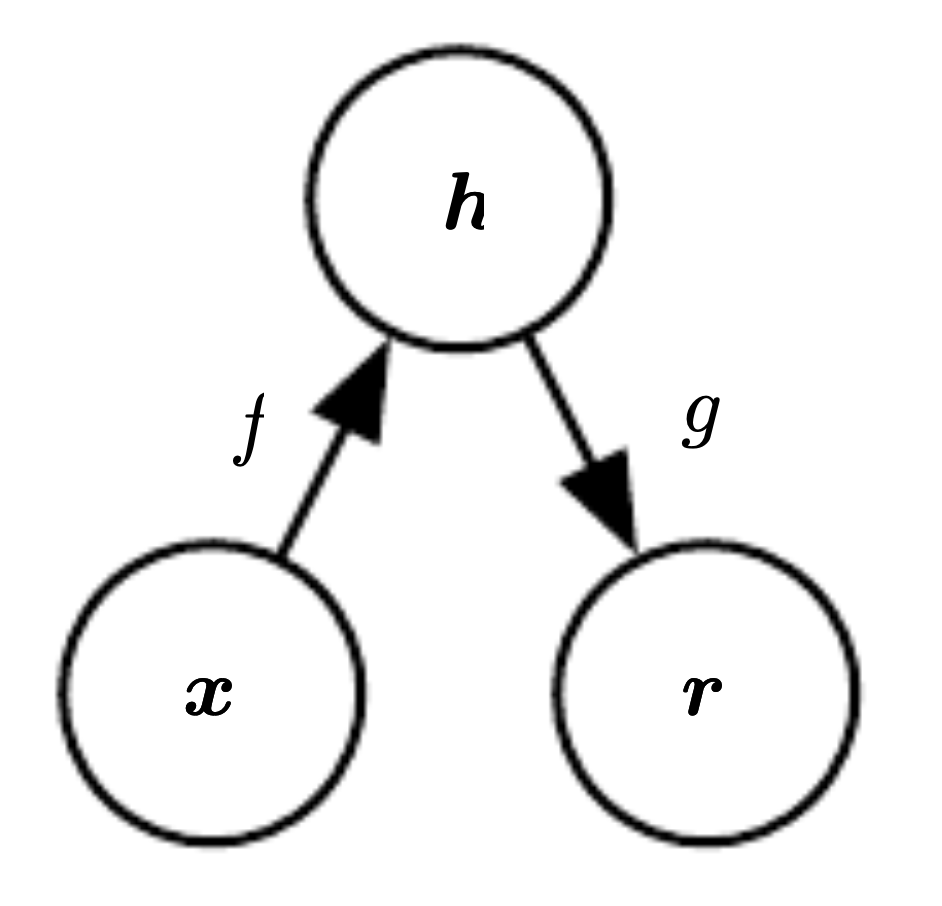
\includegraphics[width=0.3\textwidth]{resources/autoencoder-graph.png}
		\caption{Загальна структура автокодера, що відображає вхід $x$ на вихід $r$ (реконструкцію) через внутрішнє представлення $h$. Автокодер складається з двох компонентів: енкодера $f$ (відображення $x$ до $h$) та декодера $g$ (відображення $h$ до $r$) \cite{Goodfellow-et-al-2016}} 
		\label{fig:autoencoder-graph}
	\end{figure}
	Якщо автоенкодеру вдається навчитися просто відтворювати $g(f(x)) = x$ для всіх прикладів, то це не має особливої користі. Тому автоенкодери зазвичай обмежують таким чином, щоб вони не могли відтворювати ідеальну копію вхідних даним. 
		
	\subsection{Автоенкодер для видалення шуму}
	Класичні автоенкодери мінімізують деяку функцію:
	\begin{equation}
		L(\boldsymbol{x}, g(f(\boldsymbol{x})))
	\end{equation}
	де $L$ це штрафна функція яка визначає відмінність функції $g(f(\boldsymbol{x}))$ від $\boldsymbol{x}$, таку як, наприклад,  $L^{2}$ норма від їх різниці. В результаті це призводить до того, що композиція функцій $g \circ f$ навчається бути тотожнім відображення якщо для того є можливість. На відміну від цього, автоенкодер для видалення шуму мінімізує:
	\begin{equation}
		L(\boldsymbol{x}, g(f(\tilde{\boldsymbol{x}})))
	\end{equation}
	де $\tilde{\boldsymbol{x}}$ є копією $\boldsymbol{x}$ який був пошкоджений деяким шумом. 
		
	Отже, такий автоенкодер має не просто відтворити вхідні дані, а ще й відновити пошкодження. Процес тренування автоенкодера для видалення шуму заданий на \ref{fig:dae-graph}.
	\begin{figure}[h]
		\centering
		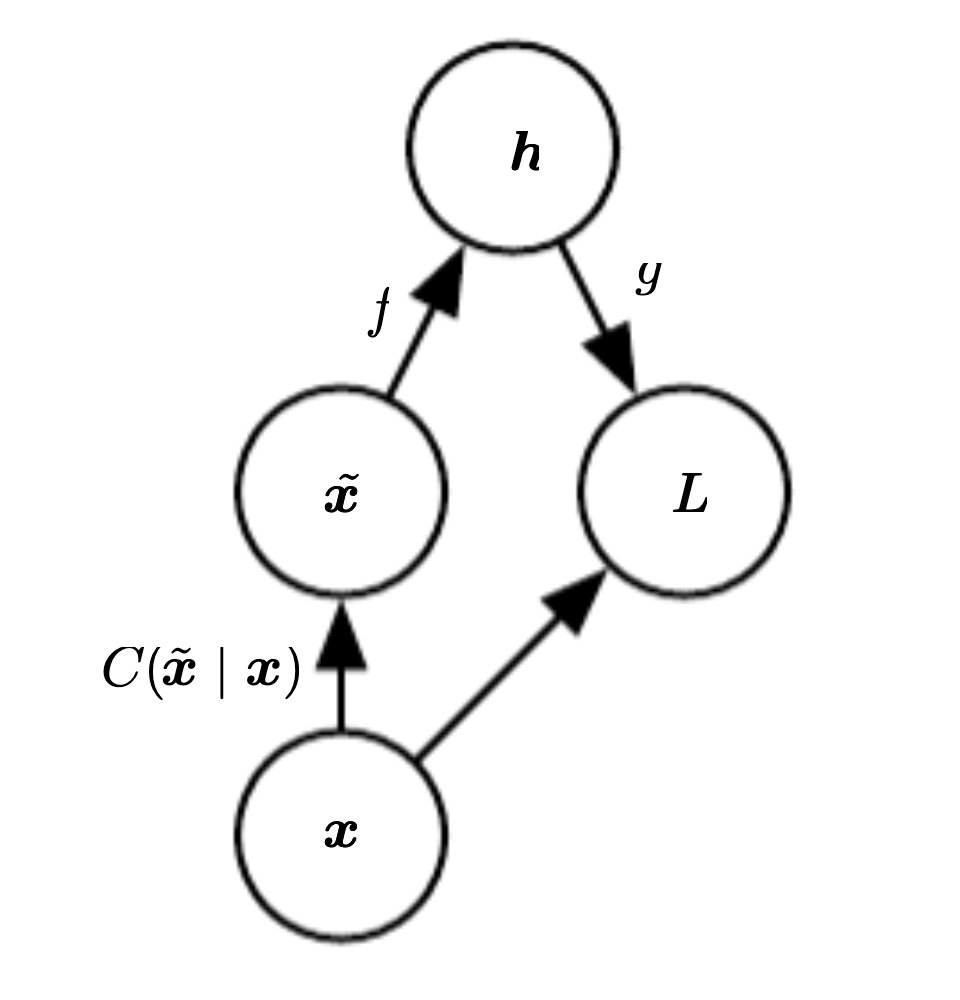
\includegraphics[width=0.4\textwidth]{resources/dae-graph.png}
		\caption{
			Структура функції витрат для автоенкодера який навчається реконстроювати чисті зображення $x$ з пошкождених. Тренування виконується на основі мінімізації функції втрат: $\tilde{x}$.  $L = - \log p (\boldsymbol {x} | \boldsymbol {h} = f (\tilde {\boldsymbol {x}}))$, де $\tilde {\boldsymbol {x}}$ - пошкоджена версія прикладу $\boldsymbol {x}$, отримана в результаті деякого процесу руйнування $C (\tilde {\boldsymbol {x}} | \boldsymbol {x})$. \cite{Goodfellow-et-al-2016}
		}
		\label{fig:dae-graph}
	\end{figure}
		
	Такий підхід до навчання видалення шуму змушує $f$ та $g$ явно вивчати структуру даних що дозволяє йому ефективно видаляти шум з пошкоджених зображень.


	%A very important property of DAEs is that their training criterion (withconditionally Gaussianp(x | h)) makes the autoencoder learn a vector field(g(f(x))− x) that estimates the score of the data distribution. This is illustratedin figure


	TODO
	Автоенкодер доцільно використовувати у випадку коли коли пряма модель $\mathcal{A}$ та чисті зображення є відомі або коли є достатня кількість пар чистих та пошкоджених зображень для тренування нейронної мережі. 


	% ============================================ %		


	\begin{comment}
	\newpage
	\thispagestyle{empty}
	\section{Варіаційний автоенкодер для розв'язування обернених задач}

	
	Ефективність автоенкодера бул суттєво покращенні з виникненням одної з його модифікацій, а саме варіаційного автоенкодеру (VAE) представленого в роботі \cite{kingma2014autoencoding}.


	\subsection{Варіаційний автоенкодер}
	
	%Нехай, енкодер приймає на вхід $x$ та повертає його приховане представлення $z$. Необхідно знайти:

	Нехай, декодер приймає на вхід приховане представлення $z$ та повертає $x$. Необхідно знайти:


	In the probability model framework, a variational autoencoder contains a specific probability model of data $x$ and latent variables $z$. We can write the joint probability of the model as $p(x, z)=p(x \mid z) p(z)$. The generative process can be written as follows.
	
	Для кожного i-ого зображення:
	- Draw latent variables $z_{i} \sim p(z)$
	- $\quad$ Draw datapoint $x_{i} \sim p(x \mid z)$

	$$
	p(z|x)=\frac{p(x|z) p(z)}{p(x)}
	$$
	Однак обчислення розподіла $p(x)$ зазвичай є обчислювально важкою задачею тому що потребує перебору всіх можливих варіантів $z$ тому обчислювати  його неоюхідно наближено. Для цього можна скористатись варіаційним висновком (variational inference). Апроксимуємо $p(z | x)$ деяким іншим розподілом $q(z | x)$, який визначимо таким чином, щоб його можна було обчислити. Якщо нам вдасться визначити параметри $q(z | x)$, щоб він був дуже близький до $p(z | x)$, ми можемо зможемо використати його для наближеного висновку про нерозв'язного розподілу.	

	\begin{defn}
		Для дискретних розподілів ймовірності $p$ та $q$ визначених на одному й тому ж імовірнісному просторі, розходженням Кульбака-Лейблера визначено як \ref{KL-divergence}.
		\begin{equation}
			\label{KL-divergence}
			D_{\mathrm{KL}}(p \| q)=-\sum_{x \in \mathcal{X}} P(x) \log \left(\frac{q(x)}{p(x)}\right)
		\end{equation}

		%Тобто, розходження Кульбака-Лейблера дає можливість визначити різницю між двома ймовірністними розподілами. 
	\end{defn}
	
	Отже для того щоб апроксимувати  $q(z | x)$  до  $p(z | x)$, необхідно мінімізувати розходження Кульбака-Лейблера для цих двохрозподілів.
	$$
	\min K L(q(z | x) \| p(z | x))
	$$
	
	
	TODO? посилання на літературу
	
	Ми можемо досягнути цього мінімізувавши наступний вираз:
	$$
		E_{q(z | x)} \log p(x | z)-K L(q(z | x) \| p(z))
	$$
	
	Перша частина формули відповідає за втрату від реконструкції. Друга частина це розбіжність між розподілами $q(z | x)$ та $p(z)$ - регуляризатор.
	
	Таким чином ми можемо використовувати $q$ для того щоб ботити висновок про можливі приховані змінні (тобто латентний стан), який був використаний для генерації спостереження. 
	
	Ми можемо далі сконструювати цю модель в архітектурі нейронної мережі, де модель кодера вивчає відображення від $x$ до $z$, а модель декодера вивчає відображення від $z$ назад до $x$.
	
	Наша функція втрат для цієї мережі складатиметься з двох частин, одна визначає розмір помилки реконструкції і друга який заохочує наш вивчений розподіл q (z | x) бути подібним істинний попередній розподіл p (z), який, як ми вважаємо, слід за одиничним розподілом Гауса для кожної розмірності j прихованого простору.
	
	
	$$
	\mathcal{L}(x, \tilde{x})+\sum_{j} K L\left(q_{j}(z \mid x) \| p(z)\right)
	$$
	
			
	\subsection{Варіаційний автоенкодер для видалення шуму}	
	відстань Кульбака — Лейблера
		
	Rather than directly outputting values for the latent state as we would in a standard autoencoder, the encoder model of a VAE will output parameters describing a distribution for each dimension in the latent space. Since we're
	
	Note: For variational autoencoders, the encoder model is sometimes referred to as the recognition model whereas the decoder model is sometimes referred to as the generative model.
	\end{comment}

	% ============================================ %		
	\newpage
	\thispagestyle{empty}
	\section{Модель глибокої нейронної мережі}

	Нехай маємо набір тренувальних даних:
	\begin{equation*}
		(x^{(1)}, y^{(1)}), \quad (x^{(2)}, y^{(2)}), \quad ... \quad ,(x^{(m)}, y^{(m)})
	\end{equation*}
	\begin{equation*}
		\quad
		x =	
		\begin{bmatrix}
			\vdots  & \vdots  & & \vdots \\
			x^{(1)} & x^{(2)} &   \dots & x^{(m)}\\
			\vdots  & \vdots  & & \vdots
		\end{bmatrix}
		\quad
		x\ith \in
		\begin{bmatrix}
			x\ith_1   \\
			\vdots \\
			x\ith_n
		\end{bmatrix}
		\quad
	\end{equation*}
	\begin{equation*}
		\quad
		y =	
		\begin{bmatrix}
			\vdots  & \vdots  & & \vdots \\
			y^{(1)} & y^{(2)} &   \dots & y^{(m)}\\
			\vdots  & \vdots  & & \vdots
		\end{bmatrix}
		\quad
		y\ith \in
		\begin{bmatrix}
			y\ith_1   \\
			\vdots \\
			y\ith_n
		\end{bmatrix}
		\quad
	\end{equation*}
	де
	\begin{itemize}
		\item $x$ - матриця в якій кожен $i-$ий стовпець є розгорнутим у вектор справжнього зображення, $i=1,\dots,m$
		\item $y$ - матриця в якії кожен $i-$ий стовпець є розгорнутим у вектор пошкодженого зображення
		\item $m$ - кількість прикладів
		\item $n$ - кількість характеристик в кожному прикладі (довжина розгорнутого в вектор зображення)
	\end{itemize}

	\subsection{Пряме поширення}
	Алгоритм прямого поширення для глибокої нейроної мереді буде мати вигляд \ref{dnn-forward-propagation}.
	\begin{equation}
		\label{dnn-forward-propagation}
		\begin{array}{l}
			\displaystyle
			z\lth=w^{(l)} a^{(l-1)}+b\lth
			\\[0.7cm]
			
			\displaystyle
			a\lth=\sigma (z\lth)
		\end{array}
	\end{equation}
	де
	\begin{itemize}
		\item $l$ - номер шару нейронної мережі, де $l = 1 \dotsc L$
		\item $n^{[l]}$ - кількість нейронів в $l$ шарі
		\item $a\lth$ - вектор стовпець активацій нейронів на для шару $l$ $(n^{[l]}$ $\cross$ 1)
		\item $b\lth$ - вектор стовпець ваг зміщення $(n^{[l]}$ $\cross$ 1)
		\item $w\lth$ - матриця ваг поміж шарами $l-1$ та $l$ $(n^{[l]} \cross n^{[l - 1]})$ 
		\item $\sigma$ - це деяка активаційна (стискуюча) функція, яку ми можемо прийняти як логістичну (для діапазону від 0 до 1) або tanh (для діапазону від -1 до 1), або будь-яку іншу диференційовану функцію.
	\end{itemize}
	
	Визначимо штрафну функцію як середньо квадратичну похибку між активаціями останнього шару $a^{(L)}$ та справжніми зображеннями $y$.
	\begin{equation}
		\label{cost-function}
		J(\omega, b) =  \frac{1}{m}  \sum_{i=1}^{m} L(a^{(L, i)}, y\ith)
	\end{equation}
	де, функцією витрати для одного набору елементів визначимо половину евклідової відстані.
	\begin{equation}
		\label{loss-function}
		L(a^{(l, i)}, y\ith)  =  \frac{1}{2}  \| a^{(l, i)}  - y\ith \|_{L_2}^{2} = \frac{1}{2} \sum_{j=1}^{n}  (a^{(l, i)}_j -  y\ith_j)^2
	\end{equation}
	де $\| \cdot \|$ це $L_2$ норма.

	\subsection{Зворотнє поширення}
	
	Задача полягає в тому, щоб знайти параметри $w \in \mathbb{R}^{m}, b\in \mathbb{R}$ що мінімізують штрафну функці реконструкції:
	\begin{equation}
		\arg \min_{w, b} J (w, b)
	\end{equation}
	Мінімізацію будемо проводити алгоритмом градієнтного спуску. Для цього, спочатку обчислюємо похідну від функції середньо квадратичної похибки останнього шару нейронної мережі.
	\begin{equation}
		\begin{array}{l}
			\displaystyle
			da^{(L, i)}
			=
			\pdv{L(a^{(L, i)}, y\ith)}{a^{(L, i)}}
			=
			\sum_{j=1}^{n}{(a^{(L, i)}_j - y\ith_j)}
			\\[0.7cm]

			\displaystyle
			dz^{(L, i)}
			=
			\pdv{L(a^{(L, i)}, y\ith)}{z^{(L, i)}}
			= 
			\pdv{L(a^{(L, i)}, y\ith)}{a^{(L, i)}} \pdv{a^{(L, i)}}{z^{(L, i)}}
			=
			\sum_{j=1}^{n}{(a^{(L, i)}_j - y\ith_j)} \sigma^{\prime}(z^{(L, i)});
			\\[0.7cm]

			\displaystyle
			dw^{(L, i)} 
			=
			\pdv{L(a^{(L, i)}, y\ith)}{w^{(L, i)}}
			=
			dz^{(L, i)} \pdv{z^{(L, i)}}{w^{(L, i)}}
			=
			dz^{(L, i)} a^{(L-1, i)};
			\\[0.7cm]
	
			\displaystyle
			db^{(L, i)}
			=
			\pdv{L(a^{(L, i)}, y\ith)}{b^{(L, i)}}
			=
			dz^{(L, i)} \pdv{z^{(L, i)}}{b^{(L, i)}} 
			= 
			dz^{(L, i)}
			\\[0.7cm]
		\end{array}
	\end{equation}

	\begin{comment}
			\displaystyle
			\pdv{a^{(L, i)}}{z^{(L, i)}}
			=
			\sigma^{\prime}(z^{(L, i)});
			\quad
			\pdv{z^{(L, i)}}{w^{(L-1, i)}}
			=
			a^{(L-1, i)};
			\quad
			\pdv{z^{(L, i)}}{b^{(L, i)}}
			=
			1;
	\end{comment}

	Перепишемо похідні в більш компактному вигляді, для всіх шарів нейронної мережі:
	\begin{equation}
		\begin{array}{l}
			\displaystyle
			\frac{\partial J(w, b)}{\partial W^{(l)}} =\frac{1}{m} \sum_{i}^{m} 	\delta^{(l, i)}\left(a^{(l-1, i)}\right)^{\top}
			\\[0.7cm]
	
			\displaystyle
			 \frac{\partial J(w, b)}{\partial b^{(l)}} =\frac{1}{m} \sum_{i}^{m} \delta^{(l, i)}
		\end{array}
	\end{equation}
	де
	\begin{equation}
		\begin{array}{l}
		\displaystyle
			\delta^{(l, i)}
			=
			\left\{
			\begin{array}{l}
				\displaystyle
				\sum_{j=1}^{n}{ \left(a^{(L, i)}_j - y\ith_j\right)} \sigma^{\prime}(z^{(L, i)}), \quad \text{якщо } l = L
				\\[0.7cm]
				
				\displaystyle
				\left((W^{(l)})^{\top} \delta^{(l+1, i)} \right) \sigma^{\prime} (z^{(l, i)}), \quad \text{якщо } l < L
			\end{array}\right.
		\end{array}
	\end{equation}

	В залежності від активаційної функції визначеної на певному шарі нейронної мережі значення похідної буде відрізнятись. Розглянемо наступні варіанти активаційних функцій:
	\begin{itemize}	
		\item \textbf{Sigmoid} (Logistic function)
		\label{sigmoid}
		\begin{equation}
			\begin{array}{l}
				\displaystyle
				\sigma(z)=\frac{1}{1+e^{-z}} \\[0.5cm]

				\displaystyle
				\sigma^{\prime}(z)=a(1-a)
			\end{array}
		\end{equation}
		
		\item \textbf{ReLU} (Rectified Linear Units)
		\begin{equation}
			\label{relu}
			\begin{array}{l}
				\displaystyle
				\sigma(z)=\max (0, z) \\[0.5cm]

				\displaystyle
				\sigma^{\prime}(z)=\left\{\begin{array}{l}
					0, z<0 \\
					1, z \geq 0
				\end{array}\right.
			\end{array}
		\end{equation}
		
		\item \textbf{Tanh} (Hyperbolic tangent)
		\begin{equation}
			\label{tanh}
			\begin{array}{l}
				\displaystyle
				\sigma(z)=\frac{e^{z}-e^{-z}}{e^{z}+e^{-z}} \\[0.5cm]

				\displaystyle
				\sigma^{\prime}(z)=1-a^{2}
			\end{array}
		\end{equation}
	\end{itemize}
	
	\begin{comment}
	\section{Датасет}
	В якості тренувального датасету будемо використовувати MNIST базу даних яка складається з 60 тис. тренувальних та 10 тис. тестувальних зображень рукописних цифр \ref{fig:minist_dataset}. Розмір кожного із них складає $28 \times 28$, а значення їх пікселів знаходяться в проміжку $[0, 255]$. На основі неї будемо здійснюватись тренування моделі і аналіз методів атак та захисту.
	\end{comment}

	Далі запишемо алгоритм заворотнього поширення з використанням стохастичного градієнтного спуску та minibatch оптимізації \ref{alg:gradient-descent}.
	\begin{algorithm}[H]
		\caption{Градієнтний спуск}
		\label{alg:gradient-descent}
		\begin{algorithmic}[1]
			\State \algorithmicrequire{Тренувальні дані $x, y$, гіперпараметри: $N$, $M$, $\varepsilon$, $\alpha$}
			\State \algorithmicensure{ Оптимальні параметри моделі $w, b$}
			\State $i = 0$
			\While{ i $< N$ or ( $\|d\omega\| < \varepsilon$ and $\|db\| < \varepsilon$ )}
			\State $x^M \leftarrow$ випадкова група прикладів $x$, розміром $M$
			\State $y^M \leftarrow$ випадкова група прикладів $y$, розміром $M$
			\For{ $l = 1$ to $L$ }
			\State $\displaystyle w^{(l)} = w^{(l)} -  \alpha \pdv{J(w, b, x^M, y^M)}{w^{(l)}}$
			\vspace{0.2cm}
			\State $\displaystyle b^{(l)} = b^{(l)} - \alpha \pdv{J(w, b, x^M, y^M)}{b^{(l)}}$
			\State $\displaystyle i = i + 1$
			\EndFor
			\EndWhile
			\State \algorithmreturn{$w, b$}.
		\end{algorithmic}
	\end{algorithm}

	% ============================================ %
	\newpage
	\thispagestyle{empty}
	\section{Генерація та оцінка шуму в зображеннях}

	\subsection{Герерація шуму}	
	Для того щоб застосувати описані методи видалення шуму, необхідно спочатку визначити яким чином цей шум, тобто прямий оперетор $\mathcal{A}$ вибрати. Для цього будемо використовувати адитивний білий гаусівський шум з різними параметрами середньокватдатичного відхилення. Задамо загальну модель адитивного шуму як \ref{additive-noise}.
	\begin{equation}
		\label{additive-noise}
		\mathbf{y}=\mathbf{x} + \mathbf{\varepsilon}
	\end{equation}
	де $\varepsilon$ це шум який має нульове середє значення та відповідає нормальному розподілу Гауса:
	\begin{equation}
		\varepsilon_{i} \sim \mathcal{N}\left(0, \sigma^{2}\right) .
	\end{equation}
	
	Ми можемо змоделювати чисте від шумів зображення $\mathbf{x} \in \mathbb{R}^{т}$ як розподіл Гауса з нульовою дисперсією, тобто $\mathbf{x}_{i} \sim \mathcal{N}(\mathbf{x}, 0)$, що дає нам змогу подати $\mathbf{y}$ теж як розподіл Гауса. Сума двох розподілів Гауса $y_{1} \sim \mathcal{N}\left(\mu_{1}, \sigma_{1}^{2}\right)$ та $y_{2} \sim \mathcal{N}\left(\mu_{2}, \sigma_{2}^{2}\right)$ також є розподілом Гауса $y_{1}+y_{2} \sim \mathcal{N}\left(\mu_{1}+\mu_{2}, \sigma_{1}^{2}+\sigma_{2}^{2}\right)$. Таким чином, шумні  вимірювання $y_{i}$ будуть відповідати по-піксельному нормальному розподілу:
	\begin{equation}
		p\left(\mathbf{y}_{i} \mid \mathbf{x}_{i}, 		\sigma\right)=\frac{1}{\sqrt{2 \pi \sigma^{2}}} e^{-\frac{\left(\mathbf{y}_{i}-\mathbf{x}_{i}\right)^{2}}{2 \sigma^{2}}}
	\end{equation}
	
	де $i = 1\dotsc n$ та $n$ - кількість пікселів. Після додавання шуму до зображення необхідно також виконати по-піксельне обрізання так, щоб$x_i \in [0, 1]$, тобто значення не виходили за межі оригінального зображення.
	%Більше про шум:
	%https://stanford.edu/class/ee367/reading/lecture10_notes.pdf
	
	\subsection{Оцінка зображень}
	Для аналізу отриманих результатів необхідно мати метрики того, наскільки зображення оброблені алгоритмом видалення шуму,  відрізняються від оригінальних зображень. Очевидним варіантом є використання середньо квадратичної похибки, яка також використовувалась у штрафній функції нейронної мережі.
	\begin{equation}
		M S E(x, y) =\frac{1}{n^2} \sum_{i=0}^{n-1} \sum_{j=0}^{n-1}[x(i, j)-y(i, j)]^{2}
	\end{equation}
	де $x$ та $y$ відповідає зображеннями розміром $n \cross n$.
	
	Однак, зазвичай, така метрика є не найкращим відображення людського сприйнятя зображень. Більш об'єктивною альтернативоє є SSIM (structural similarity index measure) метрика яка була предстадставлена в роботі \cite{1284395}. Вона дає можливіть краще оцінити схожість двох зображень $x$ та $y$ операючись на різницю в структурі всього зображення, а не окремих пікселів. SSIM метрика задається формулою \ref{SSIM}.
	\begin{equation}
		\label{SSIM}
		\operatorname{SSIM}(x, y)=\frac{\left(2 \mu_{x} \mu_{y}+c_{1}\right)\left(2 \sigma_{x 	y}+c_{2}\right)}{\left(\mu_{x}^{2}+\mu_{y}^{2}+c_{1}\right)\left(\sigma_{x}^{2}+\sigma_{y}^{2}+c_{2}\right)}
	\end{equation}
	де
	\begin{itemize}
		\item $\mu_{x}$ середнє значення $x$
		\item $\mu_{y}$ середнє значення $y$
		\item $\sigma_{x}^{2}$ дисперсія $x$
		\item $\sigma_{y}^{2}$ дисперсія  $y$
		\item $\sigma_{x y}$ коваріація $x$ та $y$
		\item $c_{1}=\left(k_{1} L\right)^{2}, c_{2}=\left(k_{2} L\right)^{2}$ змінні для стабілізації ділення
		\item $L$ динамічний діапазон пікселів
		\item $k_{1}=0.01$ та $k_{2}=0.03$ - константи.	
	\end{itemize}
	
	Значення цієї функції змінюється в діапазоні $[-1, 1]$, де $1$ можна отримати у вападку коли зображення однакові.
	
	
	% ============================================ %	
	%https://www.researchgate.net/publication/283580757_Image_noise_removal_based_on_total_variation

	\newpage
	\thispagestyle{empty}
	\section{Реалізація моделі для автоенкодера}
	
	\subsection{Датасет}

	Тренувати модель будемо використовуючи MNIST датасет який складається з 70 тис. тренувальних рукописних цифр. Всі зображення є чорно-білими та розмір кожного із них складає $28 \times 28$ пікселів, а значення лежать в проміжку від $[0,255]$. Для пришвидшення тренуваня дані  були нормалізовані до діапазону $[0, 1]$. Весь датасет був поділений на частуну тренувальних та тестових прикладів в пропорції 90/10.
	
	
	\subsection{Архітектура автоенкодера}	

	Для роботи автоенкодера зазвичай достатньо мати по одному шару енкодера та декодера. Однак, глибокі автоенкодери мають додаткові переваги і можуть вивчати більш складні взаємозвязки даних. Можна збільшувати як глибину енкодера для покращення представлення даних, так і декодера для покращення їх відтворення. Однак, збільшення кількості шарів нейронної мережі може суттєво вплинути на час її тренування і тому необхідно вибирати їх отпимальну кількість.
		
	Важливим є також вибір розмірності кожного з шарів автоенкодера. Вхідний шар завжди має розмірність зображення, тобто для випаду нашого датасету це 784. Кількість нейронів у вихідному шарі має відповідати кількості нейронів вхідного адже ми прагнемо відновити чисте зображення. Для прихованих шарів автоенкодера, зазвичай вибирають розмір між значеннями вхідного та вихідного шару. 
	
	Ключовим гіперпараметром автоеркодера є розмір репрезентаційного шару. Від нього залажить наскільки енкодер буде компресувати вхідну інформаію, що прямо впливає на можливість її подальшого відтворення. Очевидно, що при малому розмірі цього шару модель декодер буде мати менше деталей для відтворення зображення, і як наслідок, буде давати гіршиі результати.  Однак якщо зробити його розмірність занадто великою автоенкодер може просто навчитись копіювати свої вхідні дані у вихідні, не вивчаючи властивостей даних. Такий автоенкодер буде точно реконструювати навчальні дані, але через перетреновання він не зможе коректно працювати з новими прикладами.
	
	Отже відповідно до наведених вище критеріїв була побудована наступна архітектура моделі автоенкодера, яка задана таблицею \ref{tab:autoencoder-model}.
	
	\newpage
	\begin{center}
		\begin{table}[!htbp]
			\centering
			\begin{tabular}{|c|c|}
				\hline \tabboxc{10cm}{Шар мережі (активаційна функція)}
				& \tabboxc{4cm}{Розмірність} \\
				
				\hline \multicolumn{2}{|c|}{\tabboxc{2cm}{Енкодер}} \\
				
				\hline \tabboxc{4cm}{Dense (Relu)}
				 & $784 \times 64$ \\
				
				\hline \tabboxc{4cm}{Dense (Relu)}
				& $64\times 32$ \\
				
				\hline \multicolumn{2}{|c|}{\tabboxc{2cm}{Декодер}} \\
	
				\hline \tabboxc{4cm}{Dense (Sigmoid)}
				& \tabboxc{3cm}{$32\times784$}\\
				\hline
			\end{tabular} 
			\caption{Архітектура щільної нейронної мережі для автоенкодера.}
			\label{tab:autoencoder-model}
		\end{table}
	\end{center}
	Як можна побачити для енкодера було вибрано два шари, а для декодера один. Така модель була вибрана емпірично і, як можна буде побачити далі, вона демонструє досить непогані результати по відтворенню зображень. Репрезентаційний шар складається з 32 нейронів що виявилось оптимальним значенням за критерієм точності відтворення даних та часу витраченного на тренування.
	
	\subsection{Тренування}
	Всього були натреновані п'ять моделей для різних занчень стандартного відхилення білого гаусівського шуму. Для тренування кожної з них використовувався однаковий набір гіперпараметрів які задані в таблиці \ref{tab:model-hyperparameters}.
	\begin{center}
		\begin{table}[!htbp]
			\centering
			\begin{tabular}{|c|c|c|}
				\hline \tabboxc{5cm}{Кількість ітерацій}
				& \tabboxc{5cm}{Розмір minibatch частини}
				& \tabboxc{5cm}{Швидкість навчання} \\
				
				\hline \tabboxc{5cm}{35}
				& \tabboxc{5cm}{128}
				& \tabboxc{5cm}{0.015} \\
				\hline
			\end{tabular} 
			\label{tab:model-hyperparameters}
		\end{table}
	\end{center}
	
	Окрім звичайної штрафної функції, під час тренування також використовувалась SSIM оцінка для аналізу ефективністі відтворення зображень на тестових даних що продемонстровано на графіку \ref{fig:awgn-train-ssim-comparation}.
	
	\begin{figure}[H]
		\centering
		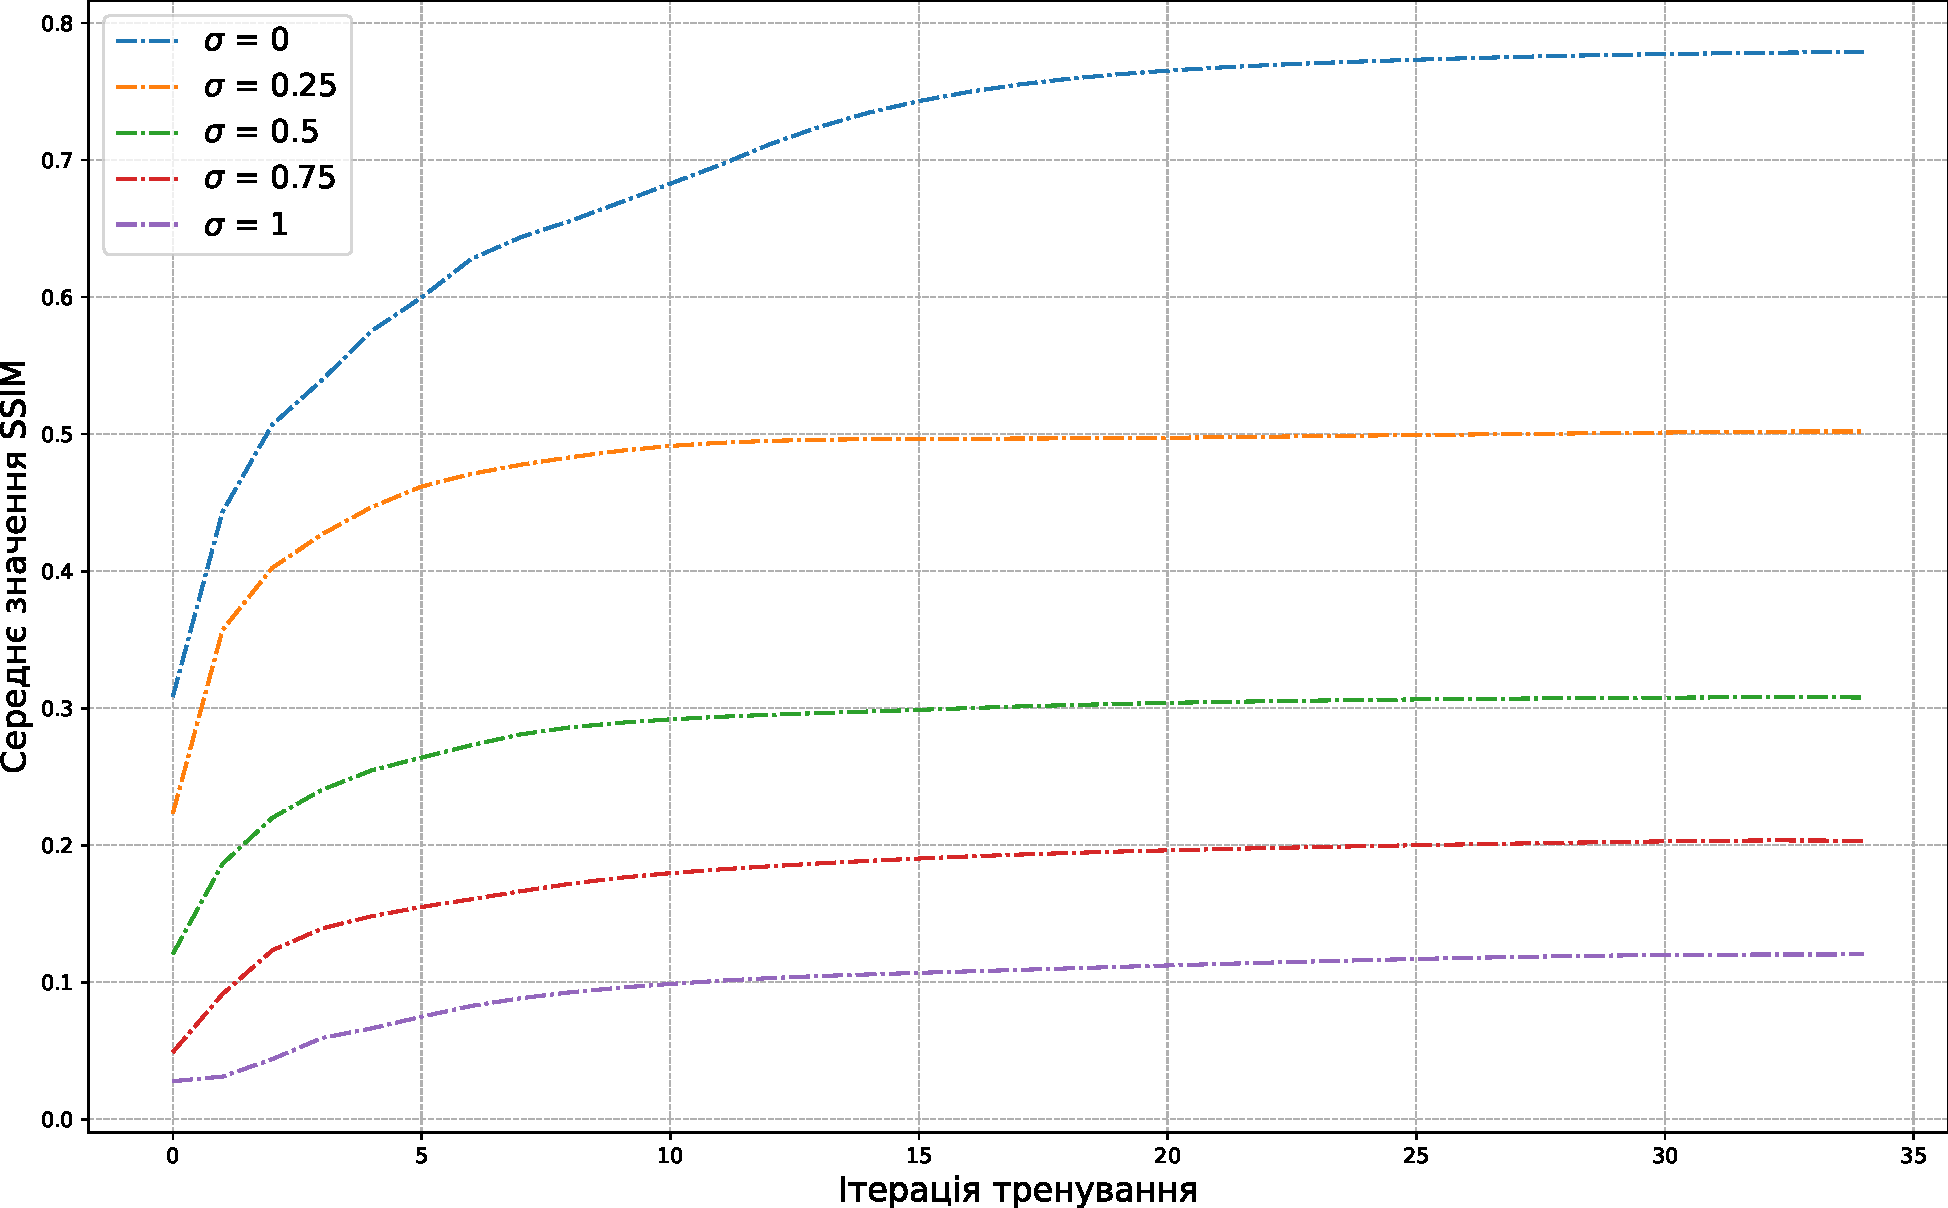
\includegraphics[width=1\textwidth]{resources/awgn-train-ssim-comparation.pdf}
		\caption{Графік залежності усередненої SSIM оцінки для тестового датасету від кількості ітерацій тренування. $\sigma$ відповідає середньоквадратичному відхиленню гаусівського шуму.}
		\label{fig:awgn-train-ssim-comparation}
	\end{figure}
	
	\begin{comment}
	\begin{figure}[H]
		\minipage[t]{0.49\textwidth}
		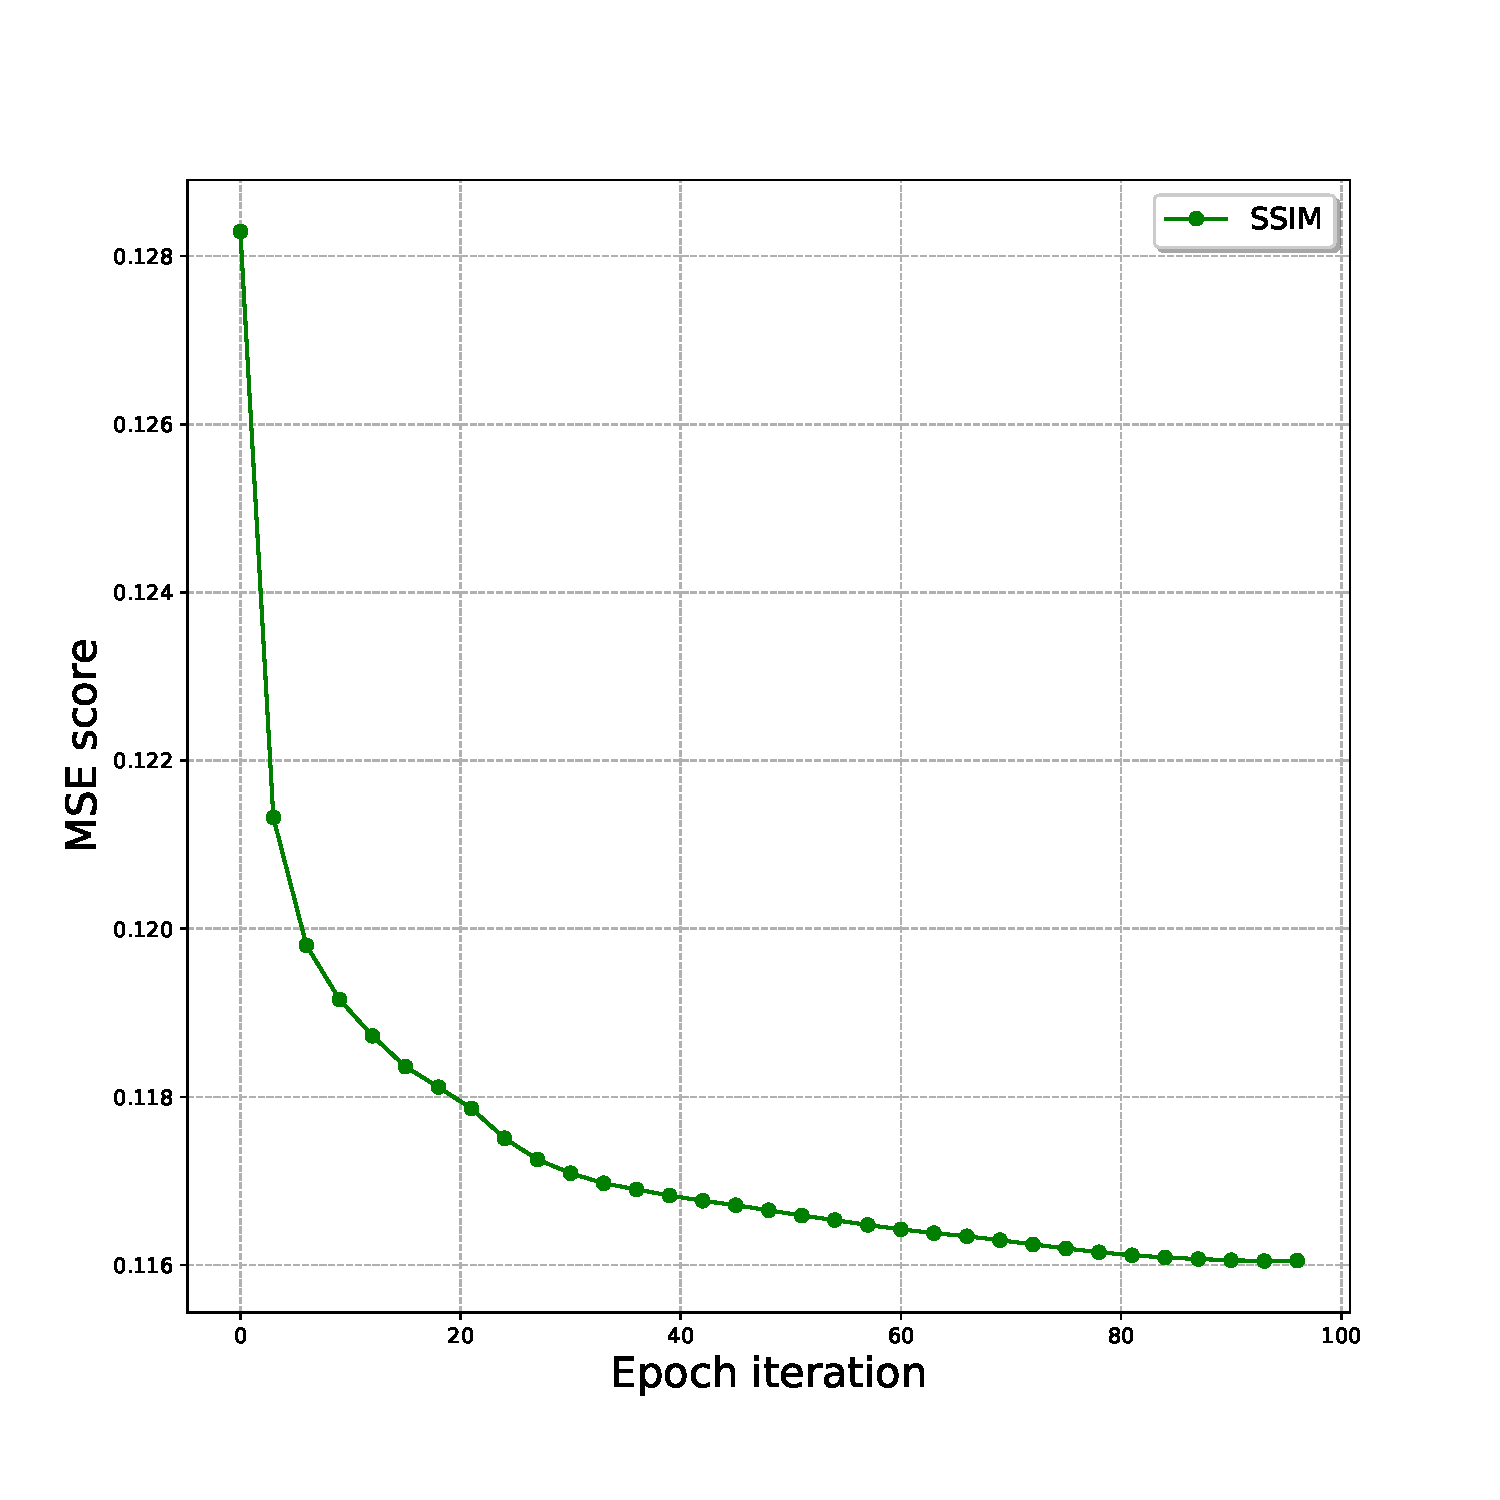
\includegraphics[width=1\textwidth]{resources/training-mse.pdf}
		\caption{Графік залежності штрафної функції MSE на тестовому датасеті від кількості епох. тренування.}
		\label{fig:attacks_bench}
		\endminipage\hfill
		\minipage[t]{0.49\textwidth}
		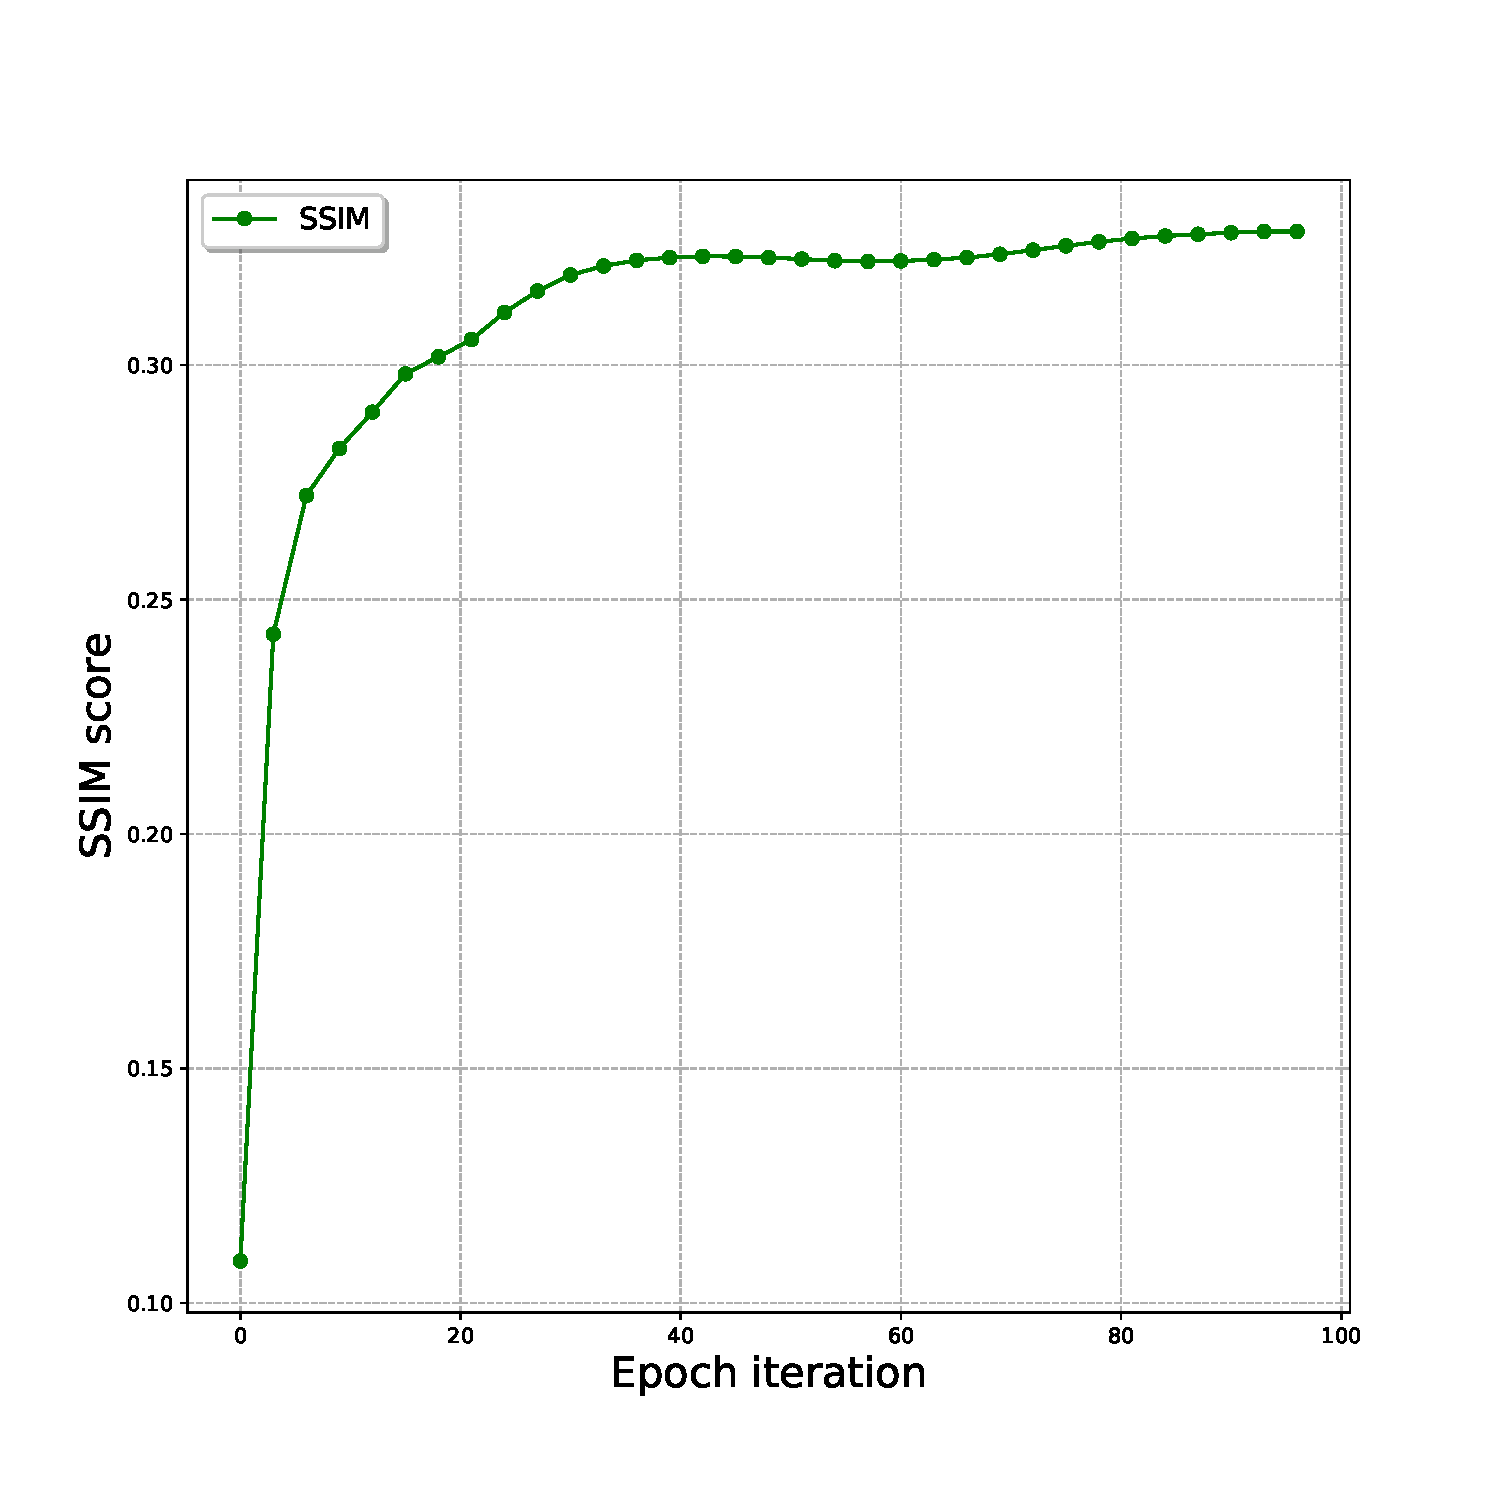
\includegraphics[width=1\textwidth]{resources/training-ssim.pdf}
		\caption{Графік залежності оцінки SSIM на тестовому датасеті від кількості епох тренування.}
		\label{fig:defenses_bench}
		\endminipage
	\end{figure}
	\end{comment}
	
	Для порівняння був також розглянутий варіант коли $\sigma = 0$. В такому випадку шум у зображення не додавався. Як можна бачити, існує чітка залежність між рівнем шуму доданим до чистих зображень та ефективністю його відтворення автоенкодером. Для $\sigma = 0$, середнє значення SSIM оцінки активно прямує до 0.8, коли для $\sigma = 1$ вона залишається в околі $0.1$.

	% ============================================ %	
		
	\newpage
	\thispagestyle{empty}
	\section{Аналіз результатів}

	Для порівняння результатів роботи автоенкодера з класичними методами був також реалізований алгоритм регуляризації Тіхонова з використанням градієнтним пріором в якості регуляризатора.
	
	\begin{figure}[H]
		\centering
		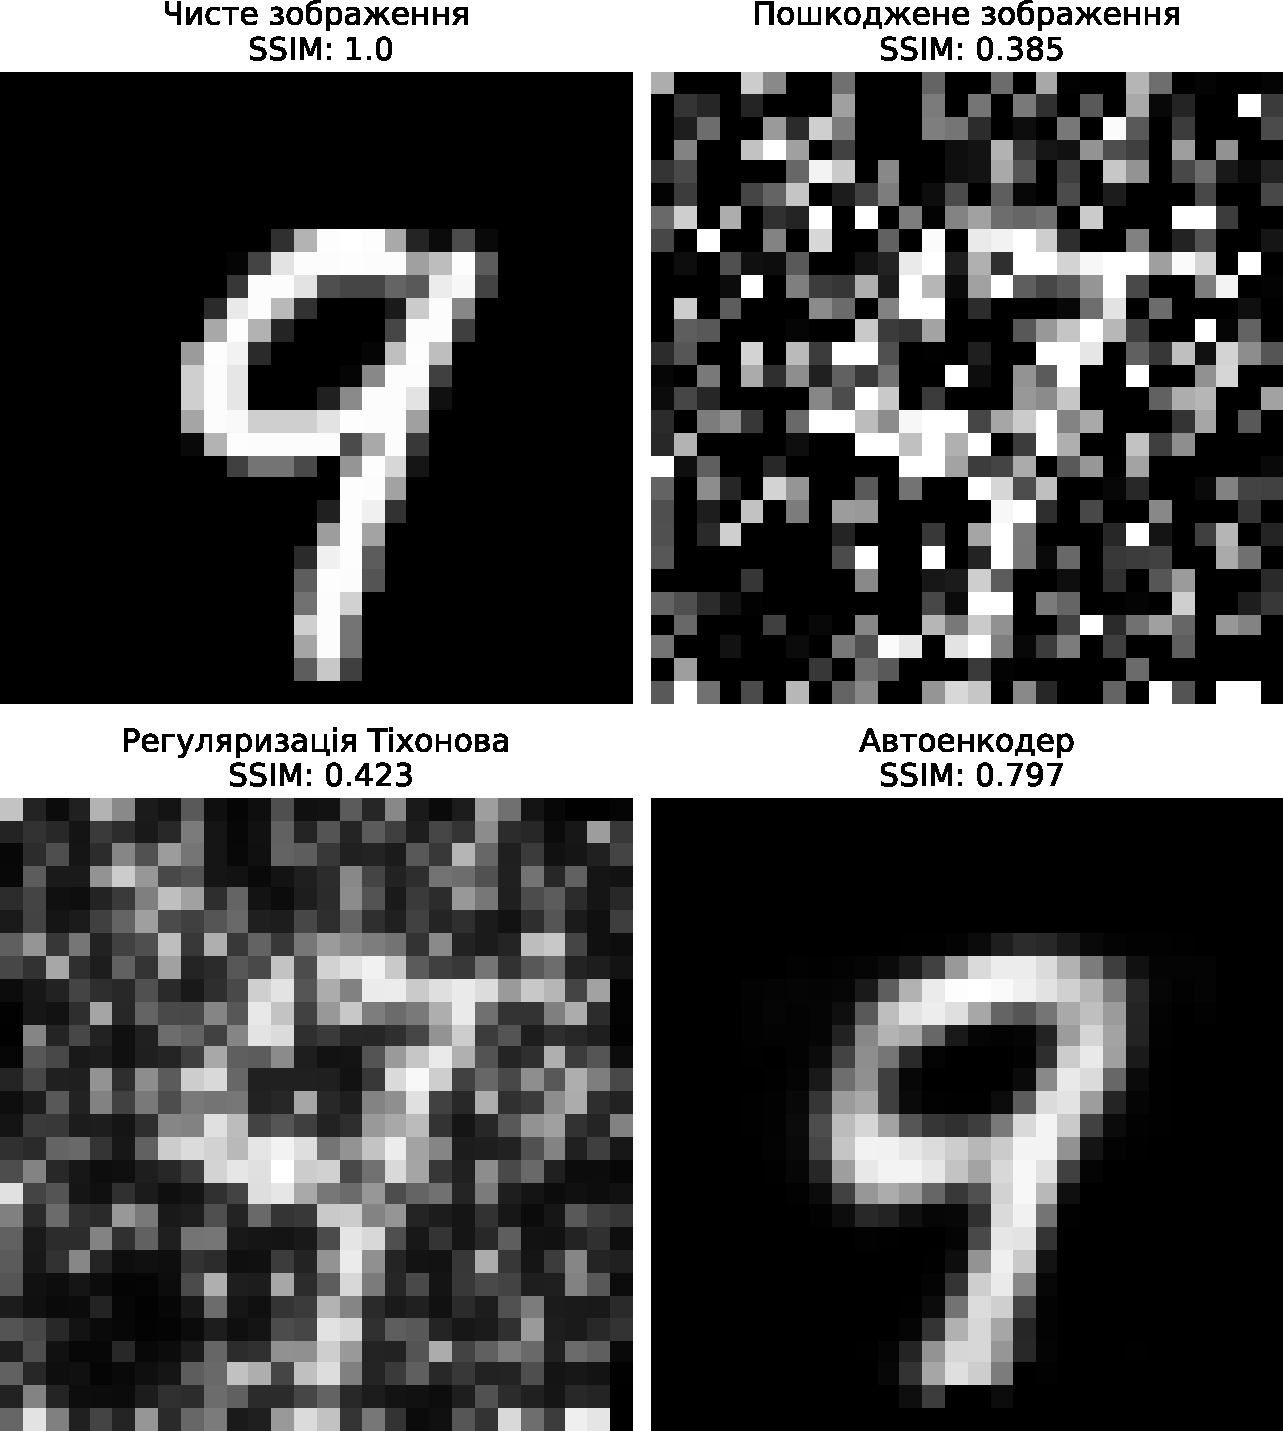
\includegraphics[width=0.8\textwidth]{resources/denoising-methods-comparation.pdf}
		\caption{}
		\label{fig:denoising-methods-comparation}
	\end{figure}
	
	Як можна бачити 
	
	
	\begin{comment}
	\begin{center}
		\begin{table}[!htbp]
			\centering
			\begin{tabular}{|c|c|c|c|}

				\hline 
				\tabboxc{6cm}{ cтандартне відхилення $\sigma$} 
				& \multicolumn{3}{|c|}{\tabboxc{6cm}{SSIM}}
				\\

				\hline
				& \tabboxc{2cm}{min} 
				& \tabboxc{2cm}{mean}
				& \tabboxc{2cm}{max}			
				\\
				
				\hline
				0.25
				& \tabboxc{2cm}{} 
				& \tabboxc{2cm}{}
				& \tabboxc{2cm}{}			
				\\

				\hline
				0.5
				& \tabboxc{2cm}{} 
				& \tabboxc{2cm}{}
				& \tabboxc{2cm}{}			
				\\

				\hline
				0.75
				& \tabboxc{2cm}{} 
				& \tabboxc{2cm}{}
				& \tabboxc{2cm}{}			
				\\

				\hline
			\end{tabular} 
			\caption{Архітектура щільної нейронної мережі для автоенкодера.}
			\label{tab:noise-comparation}
		\end{table}
	\end{center}
	\end{comment}
	
	% ============================================ %
	\newpage
	\thispagestyle{empty}
	\addcontentsline{toc}{section}{Висновок}
	\section*{Висновок}
	TODO
	
	Although deep learning is developing rapidly, it is not necessarily an effective way to solve the denoising problem. The main reason for this is that real-world denoising processes lack image pairs for training. To the best of our knowledge, the existing denoising methods are all trained by simulated noisy data generated by adding AWGN to clean images. Nevertheless, for the real-world denoising process, we find that the CNNs trained by such simulated data are not sufficiently effective.
	
	
	\newpage
	\thispagestyle{empty}
	\addcontentsline{toc}{section}{Додатки}
	\section*{Додатки}
	
	\dod{дод1}
	\begin{figure}[H]
		\centering
		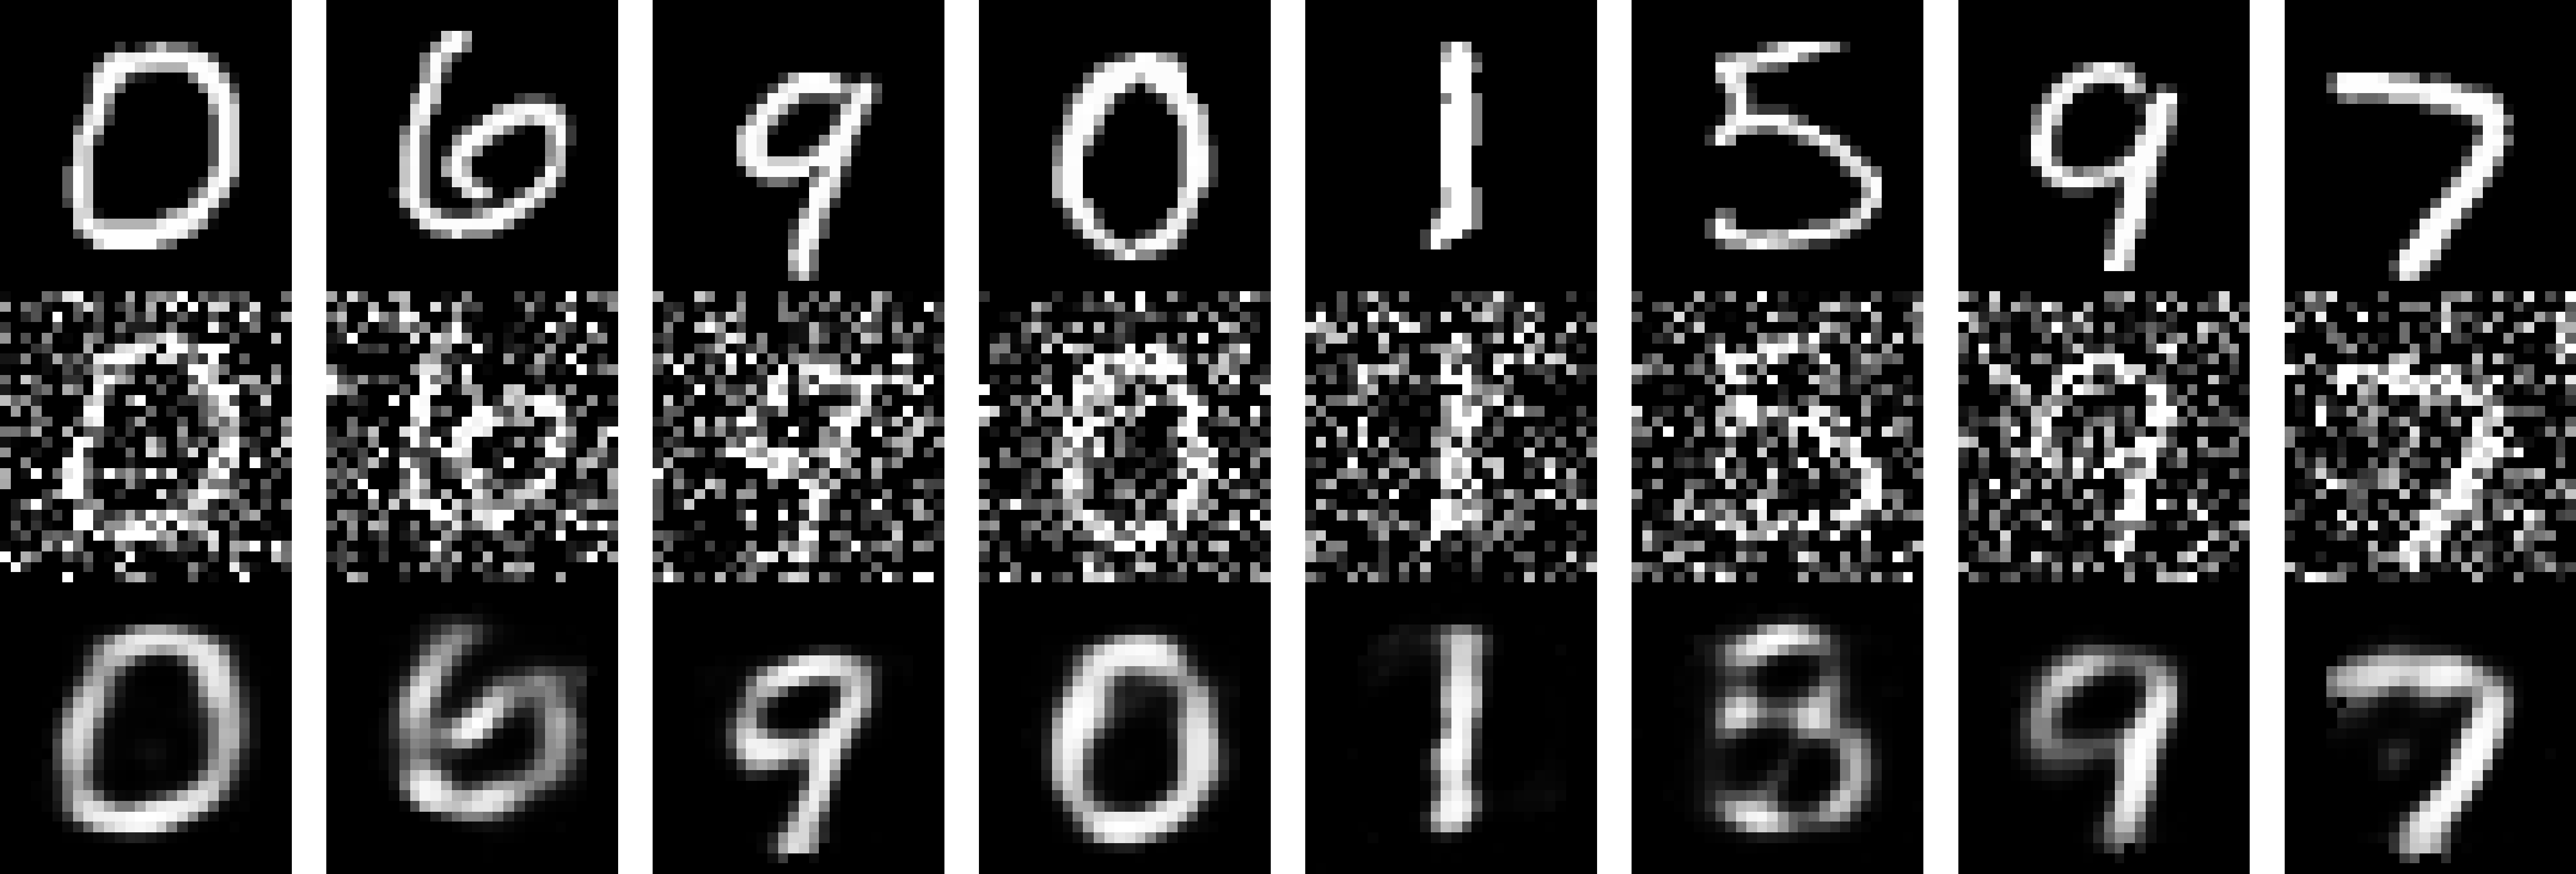
\includegraphics[width=1\textwidth]{resources/autoencoder-denoising-samples.pdf}
		\caption{Приклад видалення шуму за допомогою автоенкодера. Перший ряд чисті зображення, другий - пошкодженні, третій - відновленні}
		\label{fig:autoencoder-denoising-samples}
	\end{figure}
	
	\dod{дод2}
	\begin{figure}[H]
		\centering
		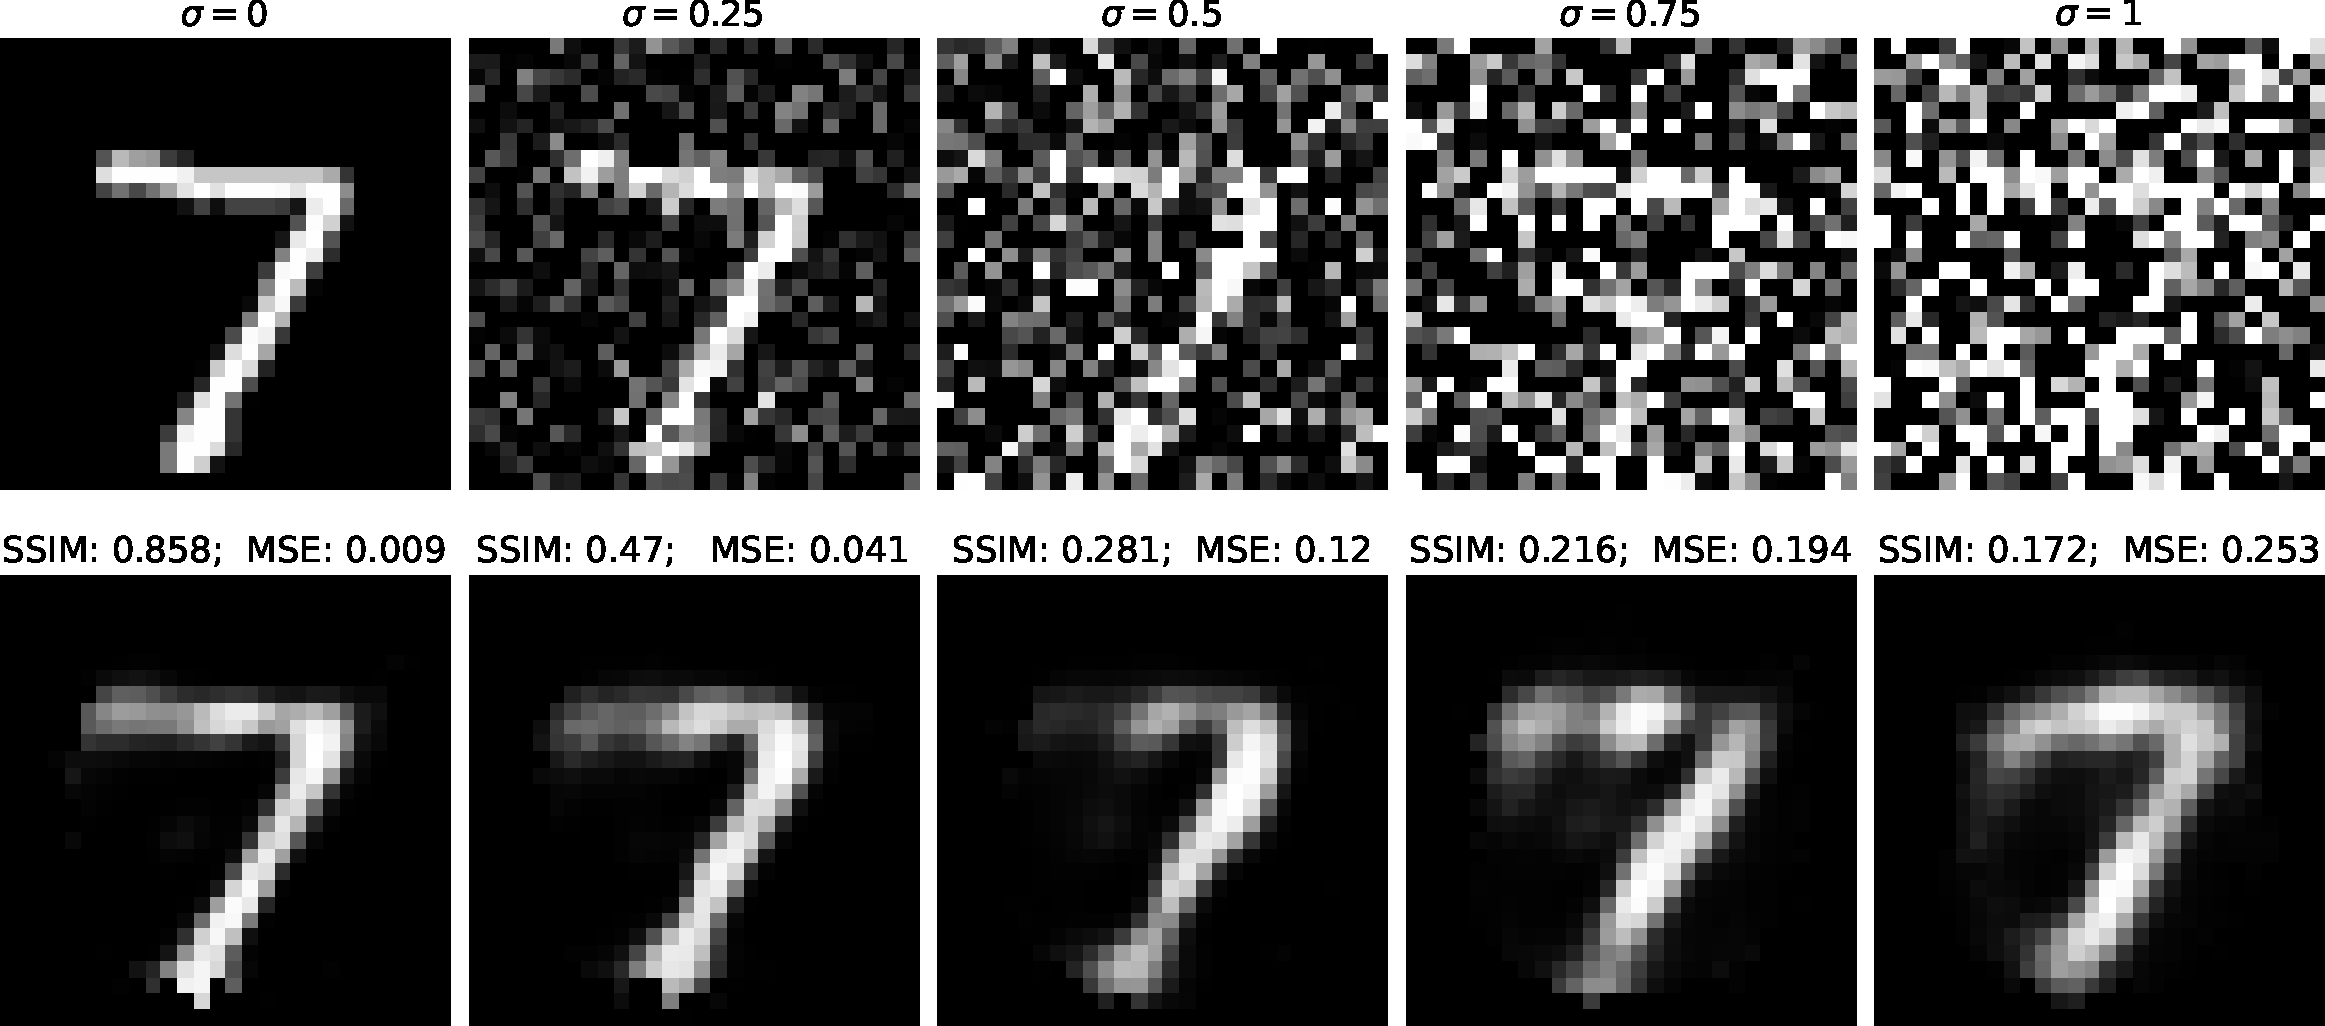
\includegraphics[width=1\textwidth]{resources/denoising-awgn-comparation.pdf}
		\caption{Порівняння }
		\label{fig:denoising-awgn-comparation}
	\end{figure}
	
	
	%============================================ %
	
	\newpage
	\thispagestyle{empty}
	\addcontentsline{toc}{section}{Література}
	
	% Deep Learning Techniques for Inverse Problems in Imaging
	\nocite{ongie2020deep}
	\nocite{Goodfellow-et-al-2016}
	\nocite{Adler_2017}
	\nocite{NIPS2012_6cdd60ea}
	\nocite{raj2019ganbased}
	\nocite{Aggarwal_2019}
	\printbibliography[title={Література}]

	https://arxiv.org/pdf/1312.6114.pdf
	https://arxiv.org/pdf/1505.03489.pdf ?
	
	% ============================================ %
\end{document}